\chapter{Архитектурные решения в мобильной разработке}

Архитектура -- это одна из важнейших частей современной разработки Android, которая определяет общую сложность кода и затраты на управление проектом.

По мере увеличения количества функций в проекте соответственно увеличиваются строки кода и его связность. Архитектура приложения в значительной степени влияет на сложность, масштабируемость и надежность вашего проекта и облегчает его тестирование. Определив границы между каждым уровнем, можно четко определить обязанности и разделить каждую ответственность, разделив их на отдельные роли.



\section{Паттерны разработки мобильного приложения}



\subsection{Шаблон проектирования Model-View-Presenter}

MVP  -- это шаблон архитектуры, который обеспечивает модульность, тестируемость и, в целом, более чистую и поддерживаемую кодовую базу (рисунок \ref{fig:MVP}) \cite{book:25}.

MVP состоит из следующих компонентов:

\begin{enumerate}
    \item model -- модель будет продолжать содержать данные в простых классах, так что здесь действительно ничего не изменится;
    \item view -- представление будет по-прежнему реализовано с использованием классов Activity или Fragment, но мы изменим область того, что контролирует представление;
    \item presenter -- этот компонент обрабатывает обновления пользовательского интерфейса на основе изменений в модели данных, а также обрабатывает вводимые пользователями данные. Презентатор будет содержать большую часть бизнес-кода.
\end{enumerate}

Данные (модель) и пользовательский интерфейс (представление) взаимодействуют друг с другом только через посредника (Presenter) \cite{book:prof}.

Презентатор содержит основную часть бизнес-логики, в то время как представление фокусируется на том, как отображать данные.

\begin{figure}[h!]
    \begin{center}
        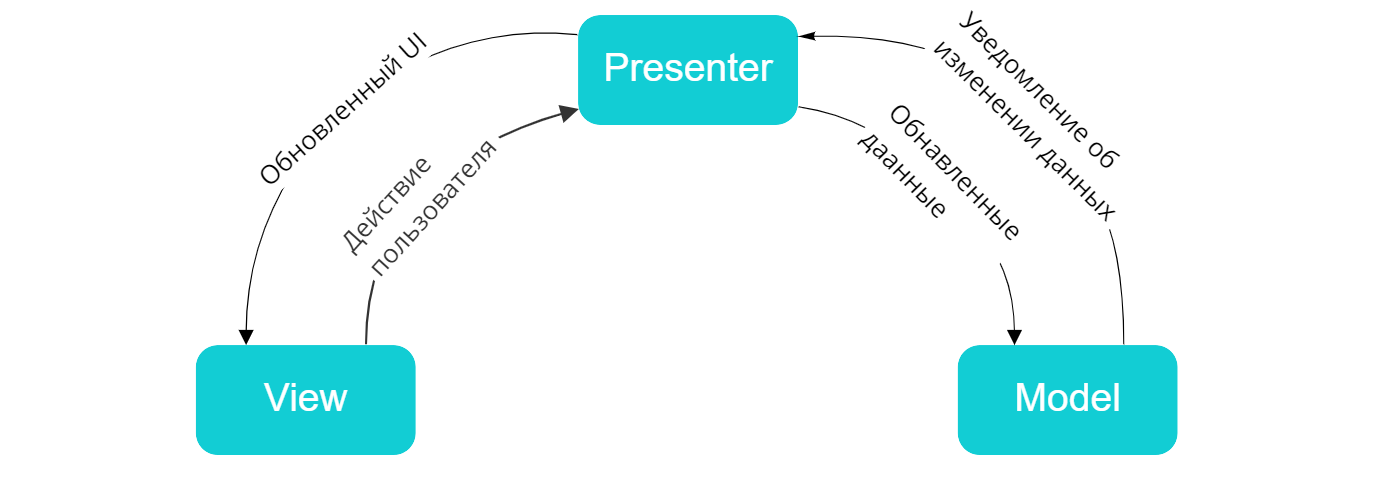
\includegraphics[width=0.95\hsize]{fig/mvp.png}\\[2mm]
        \caption{Шаблон архитектуры MVP}\label{fig:MVP}
    \end{center}
\end{figure}



\subsection{Шаблон проектирования Model-View-ViewModel}

MVVM -- это признанный в отрасли шаблон архитектуры программного обеспечения (рисунок \ref{fig:MVVM}). MVVM предлагает отделить логику представления данных от основной части бизнес-логики приложения, такое решение делает проект слабо связанным, его проще обслуживать и покрывать тестами \cite{book:21}.

В настоящее время MVVM является одним из самых популярных архитектурных проектов в современной разработке Android, поскольку Google предоставляет такие архитектурные компоненты, как ViewModel, LiveData и DataBinding.

\begin{figure}[h!]
    \begin{center}
        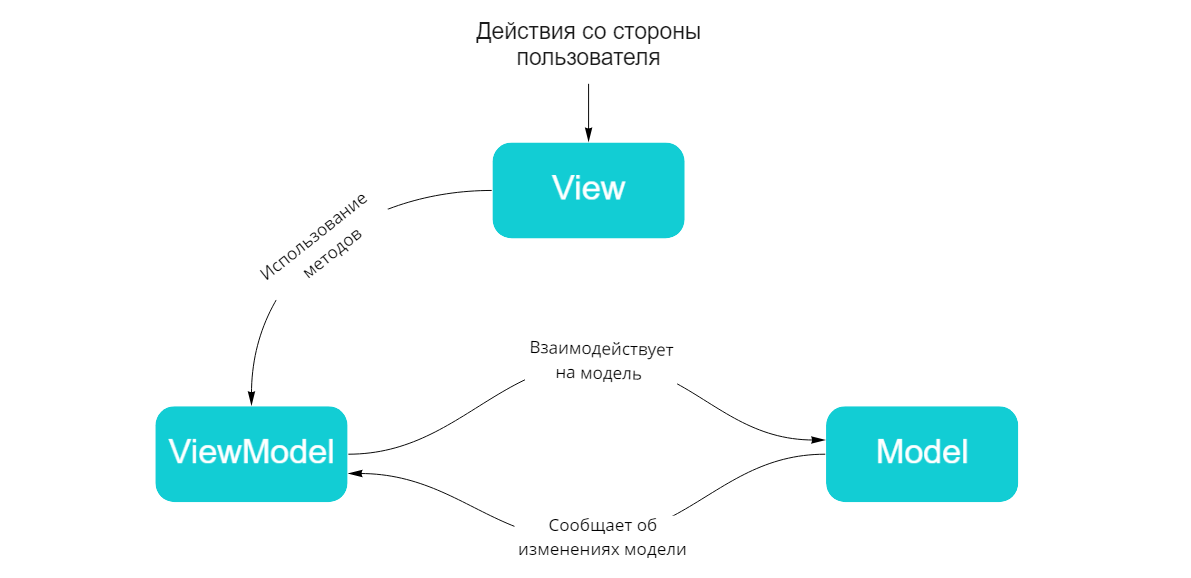
\includegraphics[width=0.95\hsize]{fig/mvvm.png}\\[2mm]
        \caption{Шаблон архитектуры MVVM}\label{fig:MVVM}
    \end{center}
\end{figure}

Каждый компонент MVVM имеет различные обязанности:

\begin{enumerate}
    \item view -- отвечает за построение пользовательских интерфейсов того, что пользователь видит на экране. Представление состоит из компонентов Android, которые включают элементы пользовательского интерфейса. Элементы пользовательского интерфейса запускают пользовательские события в ViewModel \cite{book:22}. В идеале View включает в себя только логику пользовательского интерфейса, которая представляет экран и пользовательские взаимодействия, такие как прослушиватели, и не содержит бизнес-логики;
    \item viewModel -- это независимый компонент, который не имеет никаких зависимостей от View, и он содержит бизнес-данные или состояния пользовательского интерфейса из модели для распространения их на элементы пользовательского интерфейса. Обычно существует несколько (один ко многим) отношений между ViewModel и Model, и ViewModel уведомляет об изменениях данных для просмотра в качестве данных домена или состояний пользовательского интерфейса. В современной разработке Android Google предлагает использовать библиотеку ViewModel, которая помогает разработчикам легко хранить бизнес-данные и сохранять состояния при изменении конфигурации;
    \item model -- инкапсулирует модель домена/данных приложения, которая обычно включает бизнес-логику, сложные вычислительные операции и логику проверки. Классы моделей обычно используются совместно с удаленными службами и локальными базами данных в репозиториях, которые инкапсулируют доступ к данным как набор исполняемых функций домена.
\end{enumerate}



\subsection{Шаблон проектирования Model-View-Intent}

MVI является популярной архитектурой в современной разработке Android, поскольку Jetpack Compose использует декларативное программирование (рисунок \ref{fig:MVI}) \cite{jetpack1}.

Шаблон MVI фокусируется на принципе единого источника истины для предоставления неизменяемых состояний другим слоям и однонаправленности и неизменяемости состояний, которые представляют результат действий пользователя и настраивают экраны пользовательского интерфейса \cite{book:23}.

\begin{figure}[h!]
    \begin{center}
        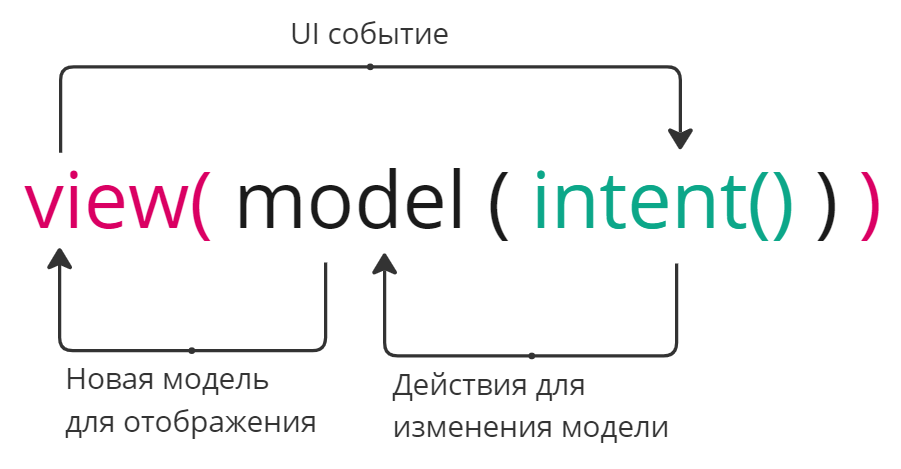
\includegraphics[width=0.95\hsize]{fig/mvi.png}\\[2mm]
        \caption{Шаблон архитектуры MVI}\label{fig:MVI}
    \end{center}
\end{figure}

MVI работает поверх других шаблонов, таких как MVP или MVVM, с механизмами управления состоянием, что означает, что архитектура MVI может использовать концепции Presenter или ViewModel в зависимости от вашего архитектурного проекта \cite{book:24}.

В отличие от MVVM и MVP, определение каждого компонента MVI немного отличается:

\begin{enumerate}
    \item intent -- намерение -- это определение интерфейсов и функций, которые обрабатывают действия пользователя. Функции преобразуют события пользовательского интерфейса в интерфейсы модели и передают результат модели для управления им. Как следует из названия, мы могли бы сказать, что у нас есть намерение выполнять функции модели;
    \item model -- модель -- это функциональный механизм, который принимает выходные данные из Intent и преобразует их в состояния пользовательского интерфейса, которые могут быть отображены в поле зрения. Состояния пользовательского интерфейса неизменяемы и исходят из бизнес-логики, которая следует единому источнику истины и однонаправленному потоку данных;
    \item view -- просмотр представляет экран и взаимодействия с пользователем и не содержит бизнес-логики. MVI обеспечивает однонаправленный поток данных, поэтому View отображает элементы пользовательского интерфейса в зависимости от состояний пользовательского интерфейса, которые поступают из модели. 
\end{enumerate}





\section{Clean Architecture метод разработки ПО}

Чистая архитектура была представлена Робертом К. Мартином в одной из его книг серии Сlean, «Clean Architecture: A Craftsman's Guide to Software Structure and Design». Он теоретизировал и представил некоторые подходы к проектированию для создания надежных и чистых архитектур для приложений, основанных на парадигмах ООП \cite{clean}. 

Чистая архитектура представляет собой подход к проектированию архитектуры программного обеспечения, который позволяет создавать приложения, котор легко тестируются, поддерживаются и масштабируются. Clean Architecture основан на нескольких ключевых принципах, таких как разделение ответственности, зависимость от абстракций, инверсия зависимостей и т.д. (рисунок \ref{fig:CleanArchScheme}).

\begin{figure}[h!]
    \begin{center}
        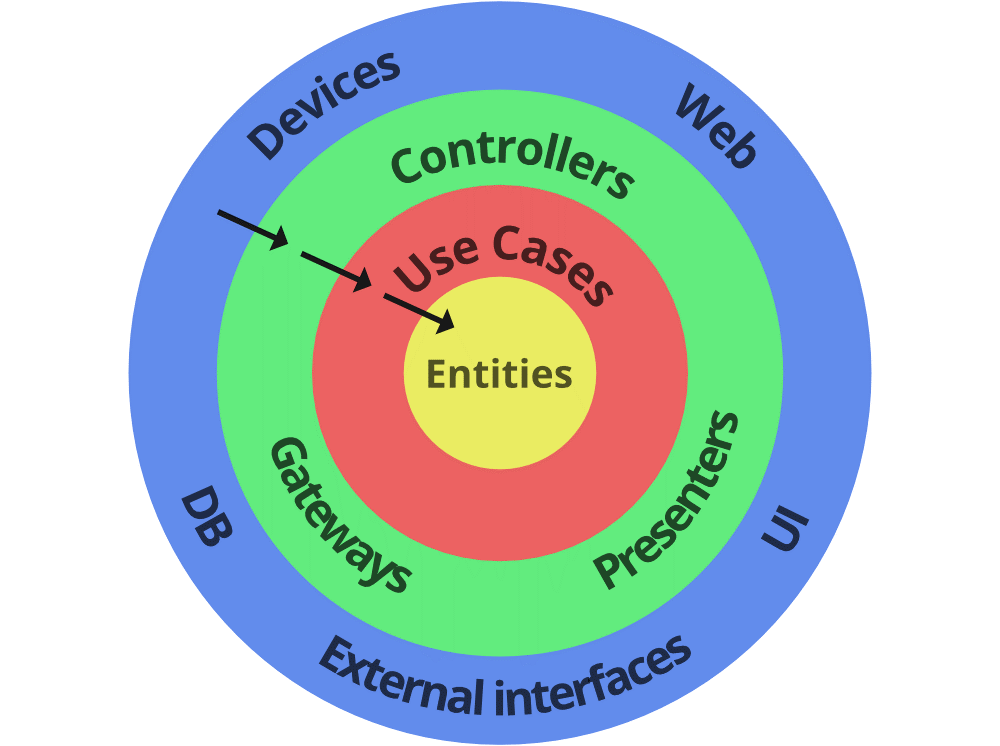
\includegraphics[width=0.45\hsize]{fig/clean.png}\\[2mm]
        \caption{Схема чистой архитектуры}\label{fig:CleanArchScheme}
    \end{center}
\end{figure}

Архитектуру можно структурно представить в виде луковицы, где зависимости идут к внутренним слоям:
\begin{enumerate}
    \item уровень сущностей. Этот уровень является самым внутренним и представлен объектами, которые содержат данные или критически важные для функции;
    \item уровень вариантов использования. Этот уровень реализует бизнес-логику системы;
    \item уровень представления. Этот уровень отвечает за преобразование данных между фреймворками, драйверами и вариантом использования. Это будет содержать такие компоненты, как ViewModels и Presenters, а также различные преобразователи, которые отвечают за преобразование сетевых данных и данных, связанных с сохранением, в объекты;
    \item уровень фреймворков и драйверов. Этот уровень является самым внешним уровнем и состоит из таких компонентов, как Activities, Fragments, сетевые компоненты и компоненты сохранения \cite{CleanArch}.
\end{enumerate}

Чистая архитектура широко используется в современной разработке Android с тех пор, как были внедрены решения для внедрения зависимостей и многомодульные проектные среды. Кроме того, эта теория может быть использована с другими архитектурами, такими как MVP, MVVM и MVI.

Современный вид Clean Architecture, использующийся в разработке мобильных приложений, является адаптацией оригинальной архитектуры Робертом К. Мартина (рисунок \ref{fig:CleanArchNEW}). Он сохраняет основные принципы оригинальной архитектуры, но включает в себя дополнительные слои и компоненты, которые учитывают специфические требования мобильных приложений:
\begin{enumerate}
    \item уровень представления. Отвечает за отображение данных пользователю и взаимодействие с пользователем. В этом слое используются паттерны MVP или MVVM для разделения логики представления от бизнес-логики;
    \item уровень домена. Отвечает за бизнес-логику приложения, в слое определяются сущности, интеракторы и репозитории;
    \item уровень данных. Отвечает за доступ к данным, в слое определяются реализации репозиториев и источников данны.
\end{enumerate}

\begin{figure}[h!]
    \begin{center}
        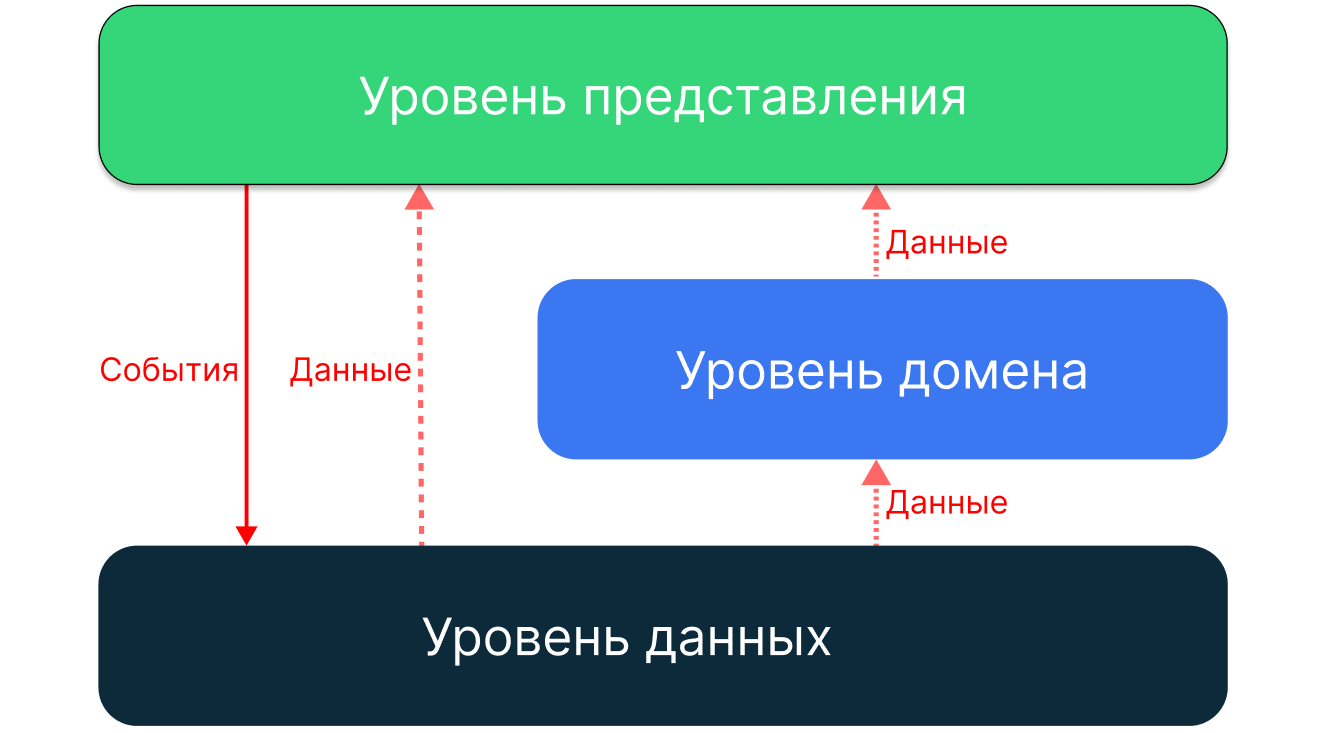
\includegraphics[width=0.65\hsize]{fig/CleanArchNEW.png}\\[2mm]
        \caption{Схема чистой архитектуры приложения}\label{fig:CleanArchNEW}
    \end{center}
\end{figure}




\section{Модульность. Решение проблемы растущей кодовой базой}

В постоянно растущей кодовой базе масштабируемость, простота чтения и общее качество кода часто снижаются с течением времени. Это происходит в результате увеличения размера кодовой базы без принятия ее сопровождающими активных мер по внедрению структуры, которую легко поддерживать. 

Модульность - это практика организации кодовой базы на слабо связанные и самодостаточные части. Каждая часть представляет собой модуль. Каждый модуль независим и служит четкой цели. Разделяя проблему на более мелкие и легко решаемые подзадачи, снижается сложность проектирования и обслуживания большой системы (рисунок \ref{fig:modul_graph}).

\begin{figure}[h!]
    \begin{center}
        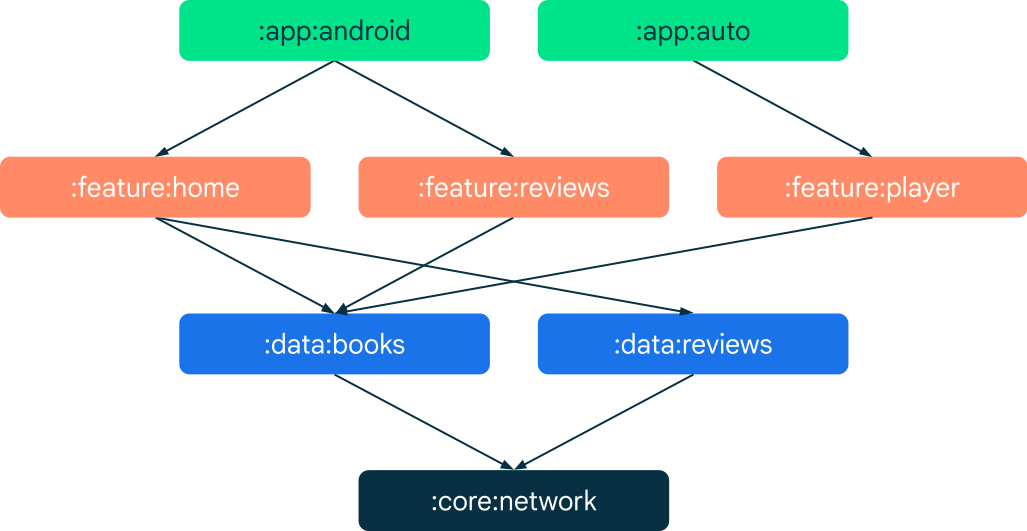
\includegraphics[width=0.95\hsize]{fig/modul_graph.png}\\[2mm]
        \caption{График зависимостей примера многомодульной кодовой базы}\label{fig:modul_graph}
    \end{center}
\end{figure}

Преимущества модульности:

\begin{enumerate}
    \item масштабируемость. В тесно связанной кодовой базе одно изменение может вызвать каскад изменений. Правильно составленный модульный проект будет основываться на принципе разделения задач;
    \item выполнение параллельной работы. Модульизация помогает уменьшить конфликты управления версиями и обеспечивает более эффективную параллельную работу разработчикам в больших командах;
    \item инкапсуляция. Изолированный код легче читать, понимать, тестировать и поддерживать;
    \item снижение связности. Низкая степень свзяности означает, что изменения в одном модуле оказывали нулевое или минимальное влияние на другие модули;
    \item возможность повторного использования. Каждый модуль может быть использован в разных частях приложения или даже в разных приложениях, что позволяет сократить время разработки и улучшить качество кода.
\end{enumerate}



Модули можно разделить на следуйщие типы:

\begin{enumerate}
    \item модули данных. Обычно содержат репозиторий, источники данных и классы моделей;
    \item функциональные модули. Изолированная часть функциональности приложения, которая обычно соответствует экрану или серии тесно связанных экранов;
    \item модули приложения. Это точка входа в приложение. Они зависят от функциональных модулей и обычно обеспечивают корневую навигацию;
    \item общие модули. Содержат код, который часто используется другими модулями. Они уменьшают избыточность и не представляют какой-либо определенный уровень в архитектуре приложения.
\end{enumerate}